\documentclass[12pt]{article}

\usepackage{amsmath, amsthm, amssymb}
\usepackage{tikz}
\usepackage{geometry}
\usepackage{float}
\usepackage{caption}
\usepackage{titlesec}
\usepackage{xcolor}
\usepackage{mdframed}
\usepackage{hyperref}

\geometry{margin=1.25in, top=1.1in, bottom=1.2in}

\hypersetup{colorlinks=false}

% Theorem styles
\theoremstyle{definition}
\newtheorem{definition}{Definition}

\theoremstyle{plain}
\newtheorem{theorem}{Theorem}

\title{\textbf{Number of Nodes in a Perfect Binary Tree}}
\author{0xHaru}
\date{\today}

\begin{document}

\maketitle

%==============================================================
\section{Definitions}
%==============================================================

\begin{definition}[Height of a binary tree]
The \textbf{height} of a binary tree is the number of edges on the
longest path from the root to a leaf.  A tree consisting of a single
node has height~$0$.
\end{definition}

\begin{definition}[Perfect binary tree]
A binary tree is \textbf{perfect} if every internal (non-leaf) node
has exactly two children and all leaf nodes reside at the same depth.
\end{definition}

\noindent
Figure~\ref{fig:perfect} shows an example of a perfect binary tree of
height~$h=3$.

\begin{figure}[H]
\centering
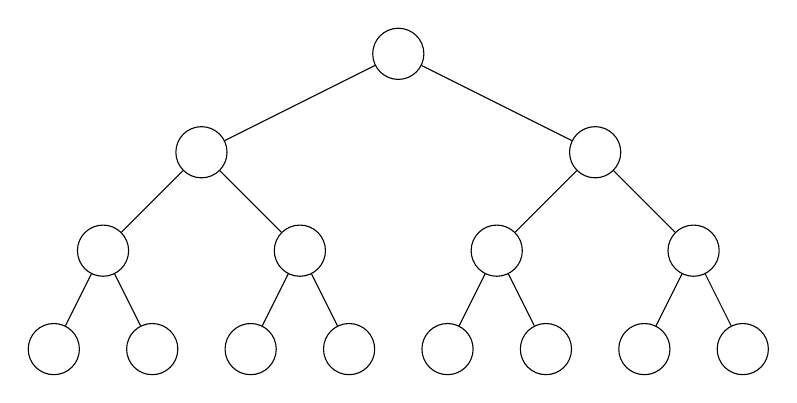
\begin{tikzpicture}[
  every node/.style={circle, draw, fill=white,
                     minimum size=6.5mm, inner sep=0pt},
  level distance=1.25cm,
  level 1/.style={sibling distance=5.0cm},
  level 2/.style={sibling distance=2.5cm},
  level 3/.style={sibling distance=1.25cm},
]
\node {}
  child { node {}
    child { node {}
      child { node {} }
      child { node {} }
    }
    child { node {}
      child { node {} }
      child { node {} }
    }
  }
  child { node {}
    child { node {}
      child { node {} }
      child { node {} }
    }
    child { node {}
      child { node {} }
      child { node {} }
    }
  };
\end{tikzpicture}
\caption{A perfect binary tree of height $h=3$.  Every internal node
  has exactly two children and all leaves sit at depth~$3$.}
\label{fig:perfect}
\end{figure}

%==============================================================
\section{Main Theorem}
%==============================================================

\begin{theorem}\label{thm:main}
A perfect binary tree of height $h \geq 0$ has exactly\/ $2^{h+1}-1$
nodes.
\end{theorem}

The two sections that follow each give a complete proof of
Theorem~\ref{thm:main}.

%==============================================================
\section{Proof 1 \textnormal{(Induction on the height)}}
%==============================================================

\begin{proof}
By induction on~$h$.  Let $N(h)$ denote the number of nodes in a
perfect binary tree of height~$h$.

\medskip
\noindent\underline{Base case ($h=0$).}\quad
A perfect tree of height~$0$ is a single root node with no children,
so
\[
  N(0)=1=2^{0+1}-1.
\]

\noindent\underline{Inductive hypothesis.}\quad
Assume, for some fixed $h\ge1$, that
\[
  N(h-1)=2^{(h-1)+1}-1=2^{h}-1.
\]

\noindent\underline{Inductive step.}\quad
We show $N(h)=2^{h+1}-1$.

\smallskip
\noindent
A perfect binary tree of height~$h$ consists of a root together with
its left and right subtrees.  Because the original tree is perfect,
each subtree is itself a perfect binary tree of height~$h-1$
(see Figure~\ref{fig:subtrees}).  Hence

\begin{align*}
N(h)
  &= \underbrace{1}_{\text{root}}
   + \underbrace{N(h-1)}_{\text{left subtree}}
   + \underbrace{N(h-1)}_{\text{right subtree}} \\[8pt]
  &= 1 + 2\,N(h-1)                              \\[6pt]
  &= 1 + 2\!\left(2^{h}-1\right)
     &&\text{(inductive hypothesis)}             \\[6pt]
  &= 1 + 2^{h+1} - 2                            \\[6pt]
  &= 2^{h+1} - 1.\qedhere
\end{align*}
\end{proof}

\begin{figure}[H]
\centering
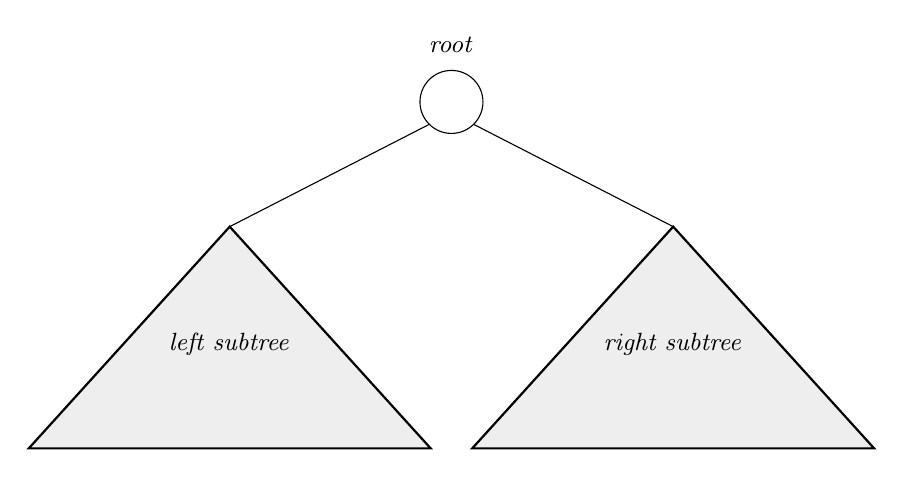
\begin{tikzpicture}[scale=0.88]
  % Root node
  \node[circle, draw, fill=white, minimum size=8mm] (root) at (0,0) {};
  \node[font=\small, above=0.1cm] at (root.north) {\textit{root}};

  % Edges to subtree apices
  \draw (root.south west) -- (-3.2, -1.8);
  \draw (root.south east) -- ( 3.2, -1.8);

  % Left subtree (filled triangle)
  \fill[gray!13] (-3.2,-1.8) -- (-6.1,-5.0) -- (-0.3,-5.0) -- cycle;
  \draw[thick]   (-3.2,-1.8) -- (-6.1,-5.0) -- (-0.3,-5.0) -- cycle;
  \node[font=\small] at (-3.2,-3.5) {\textit{left subtree}};

  % Right subtree (filled triangle)
  \fill[gray!13] ( 3.2,-1.8) -- ( 0.3,-5.0) -- ( 6.1,-5.0) -- cycle;
  \draw[thick]   ( 3.2,-1.8) -- ( 0.3,-5.0) -- ( 6.1,-5.0) -- cycle;
  \node[font=\small] at ( 3.2,-3.5) {\textit{right subtree}};
\end{tikzpicture}
\caption{A perfect binary tree of height~$h$ decomposed into its root
  and two perfect subtrees of height~$h-1$, each containing
  $N(h-1)$ nodes.}
\label{fig:subtrees}
\end{figure}

%==============================================================
\section{Proof 2 \textnormal{(Counting nodes level by level)}}
%==============================================================

\begin{proof}
The key observation — visible directly from Figure~\ref{fig:levels}
— is that each level~$k$ contains exactly $2^{k}$ nodes, so the
total is the geometric sum $\sum_{k=0}^{h}2^{k}$.  Part~1 establishes
that level count; Part~2 evaluates the sum.

\medskip
\noindent\textbf{Part 1.}\enspace\emph{Let $\ell_k$ denote the number
of nodes at level~$k$.  We show $\ell_k = 2^{k}$ by induction on~$k$.}

\medskip
\noindent\underline{Base case ($k=0$).}\quad
Level~$0$ contains exactly the root, so $\ell_0 = 1 = 2^{0}$.

\medskip
\noindent\underline{Inductive hypothesis.}\quad
Assume $\ell_k = 2^{k}$, for some $0\le k<h$.

\medskip
\noindent\underline{Inductive step.}\quad
We show $\ell_{k+1} = 2^{k+1}$.

Since the tree is perfect, every non-leaf node has \emph{exactly} two
children.  Since $k<h$, every node at level~$k$ is internal, so each
of the $\ell_k$ nodes there has exactly two children, all sitting at
level~$k+1$.
Therefore
\[
  \ell_{k+1}
    = 2\,\ell_k
    = 2 \cdot 2^{k}
    = 2^{k+1}.
\]

\noindent
Figure~\ref{fig:levels} illustrates the node counts at each level for
a perfect tree of height~$h=3$.

\medskip
\noindent\textbf{Part 2.}\enspace\emph{Summing over all levels.}

\medskip
\noindent
With Part~1 established, summing over all levels $k=0,1,\ldots,h$
gives:
\begin{align*}
\text{Total nodes}
  &= \sum_{k=0}^{h} 2^{k} \\[8pt]
  &= \frac{2^{h+1}-1}{2-1}
     && \!\!\!\left(\text{geometric series: }
        \sum_{k=0}^{n}r^{k}=\frac{r^{n+1}-1}{r-1}\right) \\[8pt]
  &= 2^{h+1}-1.\qedhere
\end{align*}
\end{proof}

\begin{figure}[H]
\centering
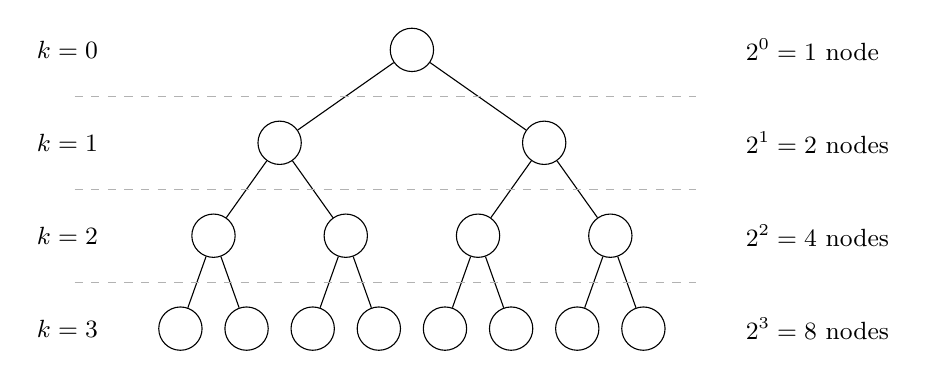
\begin{tikzpicture}[
  nd/.style={circle, draw, fill=white, minimum size=5.5mm, inner sep=0pt},
  xscale=0.84, yscale=1.18
]
  %--- Level 0 ---
  \node[nd] (a) at (4.5, 3) {};
  \node[left,  font=\small] at (-0.1, 3) {$k=0$};
  \node[right, font=\small] at ( 9.4, 3) {$2^0 = 1$ node};

  %--- Level 1 ---
  \node[nd] (b) at (2.5, 2) {};
  \node[nd] (c) at (6.5, 2) {};
  \node[left,  font=\small] at (-0.1, 2) {$k=1$};
  \node[right, font=\small] at ( 9.4, 2) {$2^1 = 2$ nodes};

  %--- Level 2 ---
  \node[nd] (d) at (1.5, 1) {};
  \node[nd] (e) at (3.5, 1) {};
  \node[nd] (f) at (5.5, 1) {};
  \node[nd] (g) at (7.5, 1) {};
  \node[left,  font=\small] at (-0.1, 1) {$k=2$};
  \node[right, font=\small] at ( 9.4, 1) {$2^2 = 4$ nodes};

  %--- Level 3 ---
  \node[nd] (h0) at (1, 0) {};
  \node[nd] (h1) at (2, 0) {};
  \node[nd] (h2) at (3, 0) {};
  \node[nd] (h3) at (4, 0) {};
  \node[nd] (h4) at (5, 0) {};
  \node[nd] (h5) at (6, 0) {};
  \node[nd] (h6) at (7, 0) {};
  \node[nd] (h7) at (8, 0) {};
  \node[left,  font=\small] at (-0.1, 0) {$k=3$};
  \node[right, font=\small] at ( 9.4, 0) {$2^3 = 8$ nodes};

  % Edges
  \draw (a)--(b);  \draw (a)--(c);
  \draw (b)--(d);  \draw (b)--(e);
  \draw (c)--(f);  \draw (c)--(g);
  \draw (d)--(h0); \draw (d)--(h1);
  \draw (e)--(h2); \draw (e)--(h3);
  \draw (f)--(h4); \draw (f)--(h5);
  \draw (g)--(h6); \draw (g)--(h7);

  % Horizontal dashed separators
  \draw[dashed, gray!60] (-0.6, 2.5) -- (8.8, 2.5);
  \draw[dashed, gray!60] (-0.6, 1.5) -- (8.8, 1.5);
  \draw[dashed, gray!60] (-0.6, 0.5) -- (8.8, 0.5);
\end{tikzpicture}
\caption{Node counts at each level in a perfect binary tree of
  height~$h=3$.  Each level~$k$ contains exactly $2^{k}$ nodes, and
  each node at level~$k$ has two children at level~$k+1$.}
\label{fig:levels}
\end{figure}

\end{document}
